\documentclass{article}
\usepackage{graphicx}
\usepackage[french]{babel}
\usepackage{float}

\title{Rapport sur l'implémentation d'agents d'apprentissage par renforcement pour le jeu Taxi-v3}
\author{Jason Perez & Samy Hadj-said}

\begin{document}

\maketitle

\section{Introduction}

Ce rapport présente l'implémentation et les résultats de trois agents d'apprentissage par renforcement pour le jeu \textit{Taxi-v3} de OpenAI Gym : \textbf{Q-Learning}, \textbf{Q-Learning avec planification d'epsilon}, et \textbf{SARSA}. L'objectif est de comparer l'efficacité des algorithmes en termes de temps d'apprentissage et de performance, tout en analysant les logs pour suivre les évolutions de performances.

\section{Choix d'implémentation}

\subsection{Q-Learning et SARSA}

Les deux algorithmes ont été implémentés avec les caractéristiques suivantes :
\begin{itemize}
    \item \textbf{Utilisation d'un dictionnaire} pour stocker les Q-valeurs, permettant une mise à jour et un accès efficaces.
    \item \textbf{Normalisation des récompenses} (division par 20) pour stabiliser l'apprentissage et éviter des mises à jour excessives.
    \item \textbf{Clipping de l'erreur TD} entre -1 et 1 pour éviter des changements brusques dans les Q-valeurs.
    \item \textbf{Stratégie d'exploration epsilon-greedy} avec une décroissance exponentielle pour le Q-Learning standard, favorisant l'exploration au début et l'exploitation à la fin.
    \item Pour SARSA, une \textbf{décroissance plus lente de l'epsilon} pour maintenir un certain niveau d'exploration plus longtemps.
\end{itemize}

\subsection{Q-Learning avec planification d'epsilon}

Cet agent étend le Q-Learning standard avec :
\begin{itemize}
    \item Une \textbf{décroissance linéaire de l'epsilon} sur un nombre fixe d'étapes, offrant un contrôle plus précis de la transition entre exploration et exploitation.
    \item Un \textbf{epsilon minimal} pour maintenir une exploration résiduelle même après la période de décroissance.
\end{itemize}

\subsection{Optimisations communes}

Pour tous les agents :
\begin{itemize}
    \item \textbf{Réinitialisation de l'agent} en cas de stagnation des performances, permettant de sortir des optima locaux.
    \item Utilisation de \textbf{moyennes mobiles} pour le suivi des performances, offrant une vue plus stable de l'évolution de l'apprentissage.
\end{itemize}

\section{Résultats et analyse des logs}

Les logs obtenus lors de l'exécution des agents montrent l'évolution des récompenses moyennes, l'amélioration continue des performances et les situations de stagnation des agents. Voici une synthèse des performances observées à partir des logs :

\subsection{Performance de l'agent Q-Learning}
\begin{itemize}
    \item Initialement, l'agent Q-Learning avait une récompense moyenne de -1955 à l'épisode 0.
    \item À l'épisode 100, la récompense moyenne s'améliore à -539, indiquant une progression continue.
    \item Après plusieurs épisodes d'entraînement, la récompense moyenne atteint 0.92 à l'épisode 1000, marquant une convergence satisfaisante des performances.
\end{itemize}

\subsection{Performance de l'agent Q-Learning avec planification d'epsilon}
\begin{itemize}
    \item La récompense moyenne de départ était de -3769 à l'épisode 0, reflétant les explorations initiales.
    \item À l'épisode 100, l'agent améliore sa récompense moyenne à -1674.
    \item Finalement, après l'épisode 1000, la récompense moyenne atteint 2.13, démontrant l'efficacité de la planification de l'epsilon dans la stratégie d'exploration.
\end{itemize}

\subsection{Performance de l'agent SARSA}
\begin{itemize}
    \item L'agent SARSA débute avec une récompense moyenne de -3132 à l'épisode 0.
    \item Au fil des épisodes, les récompenses moyennes augmentent, atteignant -6.21 à l'épisode 900.
    \item À l'épisode 1000, une récompense moyenne de 0.28 indique une stabilisation des performances et une convergence vers une politique efficace.
\end{itemize}

\section{Résultats visuels}

Les graphiques ci-dessous montrent l'évolution des récompenses totales pour chaque agent sur 1 000 épisodes :

\begin{figure}[H]
    \centering
    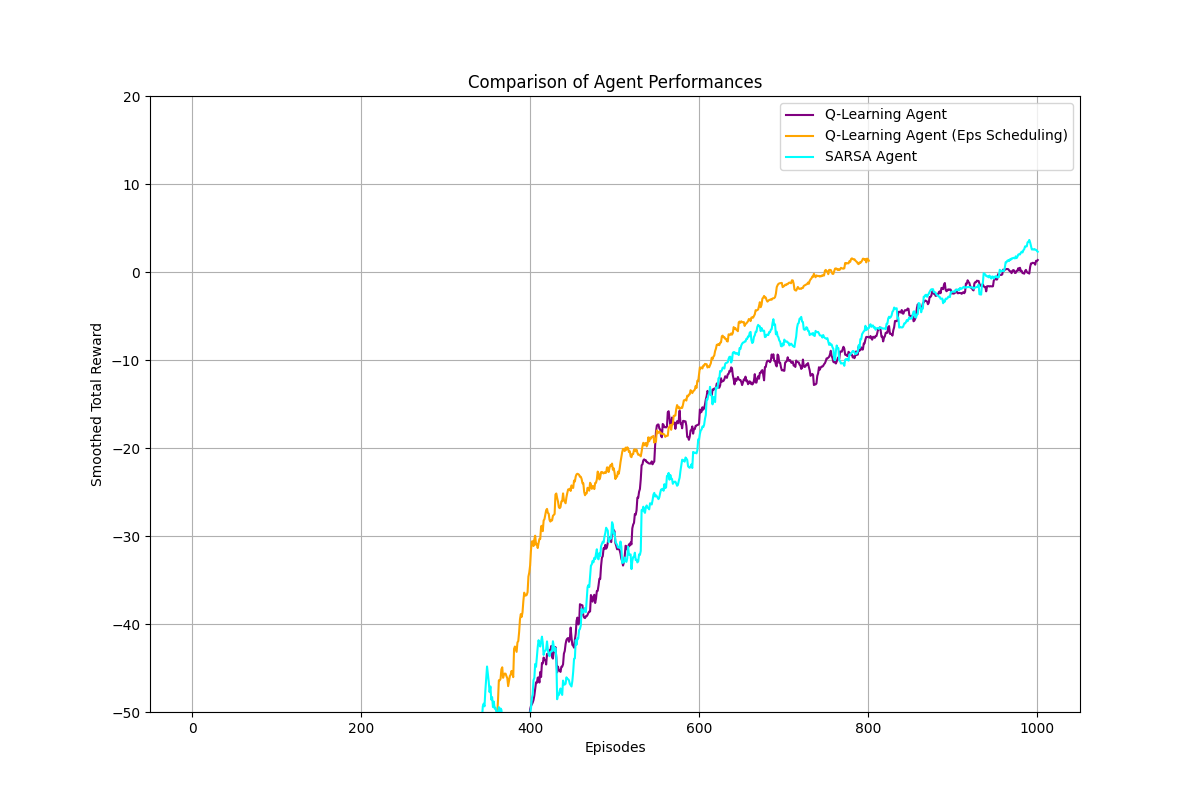
\includegraphics[width=0.8\textwidth]{imgs/ComparisonAgentPerf.png}
    \caption{Comparaison des performances des agents}
\end{figure}

\begin{figure}[H]
    \centering
    \includegraphics[width=0.8\textwidth]{imgs/QLearningAgent.png}
    \caption{Performance de l'agent Q-Learning}
\end{figure}

\begin{figure}[H]
    \centering
    \includegraphics[width=0.8\textwidth]{imgs/QLearning Eps.png}
    \caption{Performance de l'agent Q-Learning avec planification d'epsilon}
\end{figure}

\begin{figure}[H]
    \centering
    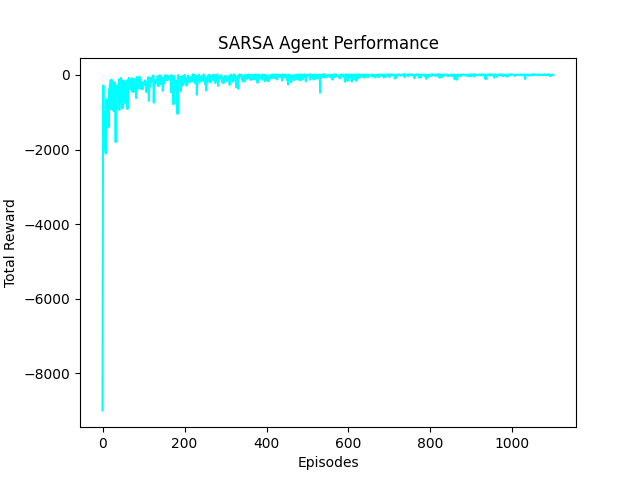
\includegraphics[width=0.8\textwidth]{imgs/SarsaAgent.png}
    \caption{Performance de l'agent SARSA}
\end{figure}

\section{Conclusion}

Les trois agents ont montré une amélioration significative de leurs performances sur le jeu \textit{Taxi-v3}, chacun suivant une dynamique d'apprentissage différente. Le Q-Learning avec planification d'epsilon a offert une convergence plus douce, tandis que l'agent SARSA a montré une convergence stable mais plus lente. Le Q-Learning standard a quant à lui démontré une montée en performance plus rapide, se montrant efficace pour ce problème spécifique.

\section{Perspectives}

Plusieurs pistes d'amélioration peuvent être explorées :
\begin{itemize}
    \item Étendre l'implémentation vers des algorithmes de type DQN pour gérer des espaces d'états plus complexes.
    \item Tester des stratégies d'exploration plus sophistiquées pour accélérer l'apprentissage.
    \item Expérimenter avec des environnements plus variés pour évaluer la capacité de généralisation des agents.
\end{itemize}

\end{document}